\documentclass[t]{beamer}

\usepackage{wrapfig}
\usepackage{float}
% For tabs in verbatim
\usepackage{fancyvrb}

% set fonts
\usefonttheme{professionalfonts} % using non standard fonts for beamer
\usepackage{txfonts,mathptmx}

% set indend spacing for first and second level indentation
\setlength{\leftmargini}{0.5cm}
\setlength{\leftmarginii}{0.5cm}
\setlength{\leftmarginiii}{0.5cm}

% Set circles for bullets 
\setbeamertemplate{itemize items}[circle]

% colors
\usepackage{xcolor}

% multiple columns
\usepackage{multicol}

% todo lists
\usepackage{pifont}
\usepackage{amssymb}

% increase space between text and frame name
\addtobeamertemplate{frametitle}{}{\vspace{0.5em}}

%Information to be included in the title page:
\title{Verilog Introduction}
\author{Nikola Petrovic}
\institute{University of Belgrade, School of Electrical Engineering}
\date{2022}



\begin{document}

\frame{\titlepage}

%%%%%%%%%%%%%%%%%%%%%%%%%%%%%%%%%%%%%%%%%%%%%%%%%%%%%%%%%%%%
\begin{frame}
\frametitle{Module Objective}

In this module we will use Verilog to describe a simple design.
\newline

\textbf{Topics}

\begin{itemize}
\item Describing design modules
\item Representing hierarchy
\item Describing module behavior
\item Synchronizing module behaviors
\item Communicating between behaviors
\item Rules for identifiers, comments, white space
\item Configuring and compiling a design
\end{itemize}

\end{frame}

%%%%%%%%%%%%%%%%%%%%%%%%%%%%%%%%%%%%%%%%%%%%%%%%%%%%%%%%%%%%
\begin{frame}[fragile]
\frametitle{Describing Design Modules}

\begin{enumerate}
\item We need to start with \textcolor{red}{module} keyword
\item \textcolor{purple}{Describe module interface}
\item \textcolor{brown}{Describe module behavior}
\item End with \textcolor{red}{endmodule} keyword
\end{enumerate}

In Verilog-2001 we can write:
\newline

\begin{Verbatim}[commandchars=\\\{\}, tabsize=2]
\textcolor{purple}{module} halfadd (
	\textcolor{purple}{input} a, b,
	\textcolor{purple}{output} sum, carry
);
	\textcolor{purple}{assign} sum   = a ^ b;
	\textcolor{purple}{assign} carry = a & b;
\textcolor{purple}{endmodule}
\end{Verbatim}

\end{frame}

%%%%%%%%%%%%%%%%%%%%%%%%%%%%%%%%%%%%%%%%%%%%%%%%%%%%%%%%%%%%
\begin{frame}
\frametitle{Creating Hierarchy}

\begin{itemize}
\item We need to declare local nets and variables
\item Instantiate module and connect its ports to the local nets and variables
\item We can connect an instance of a module using:
\begin{itemize}
	\item Named port connection.
	\item Ordered port connection.
\end{itemize}
\item We will be connecting two half-adders together:
\end{itemize}

\begin{figure}[H!]
    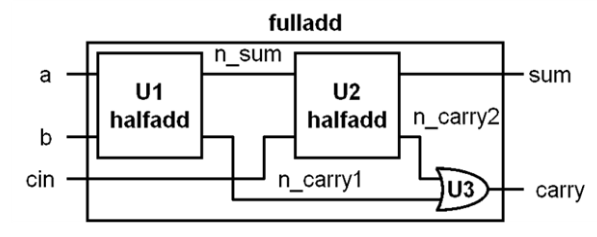
\includegraphics[width=0.5\textwidth]{img/03_fulladd.png}
\end{figure}

\end{frame}

%%%%%%%%%%%%%%%%%%%%%%%%%%%%%%%%%%%%%%%%%%%%%%%%%%%%%%%%%%%%
\begin{frame}[fragile]
\frametitle{Named port connection}
\begin{multicols}{2}
{\scriptsize%
\begin{Verbatim}[commandchars=\\\{\}, tabsize=2]
\textcolor{purple}{module} fulladd(
    \textcolor{blue}{input} a, b, cin,
    \textcolor{blue}{output} sum, carry
);
    \textcolor{blue}{wire} w_sum, w_carry1, w_carry2;
    \textcolor{blue}{halfadd U1}(
        .a(a),
        .b(b),
        .sum(w_sum),
        .carry(w_carry1)
    );
    \textcolor{blue}{halfadd U2}(
        .a(w_sum),
        .b(cin),
        .sum(sum),
        .carry(w_carry2)
    );
    \textcolor{blue}{or U3}(
        carry, 
        w_carry2,
        w_carry1
    );
\textcolor{purple}{endmodule}
\end{Verbatim}
}
\columnbreak
\begin{figure}[H!]
	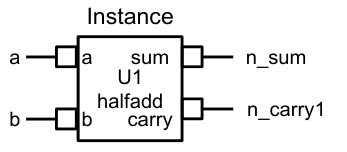
\includegraphics[width=0.35\textwidth]{img/03_inst.png}
\end{figure}
\begin{figure}[H!]
    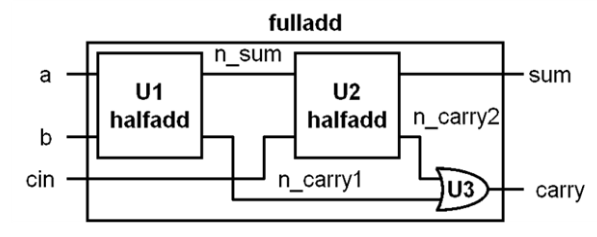
\includegraphics[width=0.35\textwidth]{img/03_fulladd.png}
\end{figure}
\end{multicols}
\end{frame}

%%%%%%%%%%%%%%%%%%%%%%%%%%%%%%%%%%%%%%%%%%%%%%%%%%%%%%%%%%%%
\begin{frame}[fragile]
\frametitle{Ordered port connection}
\begin{multicols}{2}
{\scriptsize%
\begin{Verbatim}[commandchars=\\\{\}, tabsize=2]
\textcolor{purple}{module} fulladd(
    \textcolor{blue}{input} a, b, cin,
    \textcolor{blue}{output} sum, carry
);
    \textcolor{blue}{wire} w_sum, w_carry1, w_carry2;
    \textcolor{blue}{halfadd U1}(
        a,
        b,
        w_sum,
        w_carry1
    );
    \textcolor{blue}{halfadd U2}(
        w_sum,
        cin,
        sum,
        w_carry2
    );
    \textcolor{blue}{or U3}(
        carry, 
        w_carry2,
        w_carry1
    );
\textcolor{purple}{endmodule}
\end{Verbatim}
}
\columnbreak
\begin{figure}[H!]
	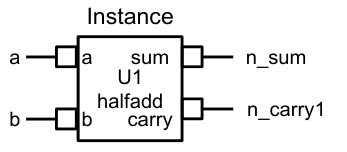
\includegraphics[width=0.35\textwidth]{img/03_inst.png}
\end{figure}
\begin{figure}[H!]
    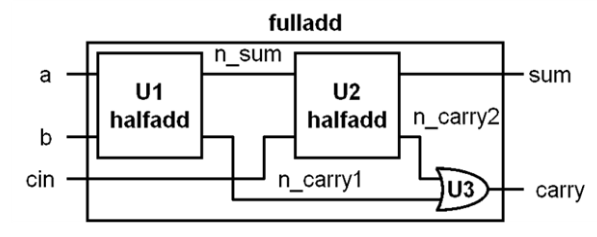
\includegraphics[width=0.35\textwidth]{img/03_fulladd.png}
\end{figure}
\end{multicols}
\end{frame}

%%%%%%%%%%%%%%%%%%%%%%%%%%%%%%%%%%%%%%%%%%%%%%%%%%%%%%%%%%%%
\begin{frame}[fragile]
\frametitle{Describing Module Behavior With Procedural Blocks}

\begin{multicols}{2}
\begin{itemize}
\item Procedural blocks start with:
\begin{itemize}
	\item \textcolor{purple}{always}
	\begin{itemize}
		\item Synthesizable construct
		\item Executes at the start of simulation
		\item Execution blocks and unblocks in accordance with timing controls
		\item When at end, loops back to beginning
	\end{itemize}
\end{itemize}
\begin{itemize}
	\item \textcolor{purple}{initial}
	\begin{itemize}
		\item Non-synthesizable  or Testbench construct
		\item Executes at the start of simulation
		\item Execution blocks and unblocks in accordance with timing controls
		\item When at end, terminates
	\end{itemize}
\end{itemize}
\end{itemize}

\columnbreak
{\footnotesize%
\begin{Verbatim}[commandchars=\\\{\}, tabsize=2]
\textcolor{purple}{always} @ (a or b or select)
\textcolor{blue}{begin}
	\textcolor{purple}{if} (select == 1)
		op = b;
	\textcolor{purple}{else}
		op = a;
\textcolor{blue}{end}



\textcolor{purple}{initial}
\textcolor{blue}{begin}
	a = 1;
	b = 0;
\textcolor{blue}{end}
\end{Verbatim}
}
\end{multicols}
\end{frame}

%%%%%%%%%%%%%%%%%%%%%%%%%%%%%%%%%%%%%%%%%%%%%%%%%%%%%%%%%%%%
\begin{frame}[fragile]
\frametitle{Describing Module Behavior With Procedural Blocks}


\begin{itemize}
\item Multiple statements are enclosed between \textcolor{purple}{begin} and \textcolor{purple}{end} keywords
\item \textcolor{red}{Multiple procedural blocks interact concurrently!!!}
\end{itemize}
\vspace{3pt}
{\scriptsize%
\begin{Verbatim}[commandchars=\\\{\}, tabsize=2]
\textcolor{purple}{always} @ (a or b or select)
\textcolor{blue}{begin}
	\textcolor{purple}{if} (select == 1)
		op = b;
	\textcolor{purple}{else}
		op = a;
\textcolor{blue}{end}

\textcolor{purple}{always} @ (posedge clock)
\textcolor{blue}{begin}
	r_counter <= r_counter + 1'b1;
\textcolor{blue}{end}
\end{Verbatim}
}

\end{frame}

%%%%%%%%%%%%%%%%%%%%%%%%%%%%%%%%%%%%%%%%%%%%%%%%%%%%%%%%%%%%
\begin{frame}[fragile]
\frametitle{Synchronizing Module Behaviors}

\begin{multicols}{2}
\begin{itemize}
\item Use the @ event control
\item Execution blocks until an event in the event expression occurs
\item An event is any transition of the specified nets and variables
\item In Verilog-2001 and above we can used commas and wildcard operators
\item Parentheses are optional for event expressions consisting of a single token
\end{itemize}

\columnbreak
\begin{itemize}
\item 1995: or operator
\end{itemize}
{\tiny%
\begin{Verbatim}[commandchars=\\\{\}, tabsize=2]
\textcolor{purple}{always} @ (a or b or select)
\textcolor{blue}{begin}
	\textcolor{purple}{if} (select == 1)
		op = b;
	\textcolor{purple}{else}
		op = a;
\textcolor{blue}{end}
\end{Verbatim}
}
\begin{itemize}
\item 2001+: comma operator
\end{itemize}
{\tiny%
\begin{Verbatim}[commandchars=\\\{\}, tabsize=2]
\textcolor{purple}{always} @ (a, b, select)
\textcolor{blue}{begin}
	\textcolor{purple}{if} (select == 1)
		op = b;
	\textcolor{purple}{else}
		op = a;
\textcolor{blue}{end}
\end{Verbatim}
}
\begin{itemize}
\item 2001+: wildcard operator
\end{itemize}
{\tiny%
\begin{Verbatim}[commandchars=\\\{\}, tabsize=2]
\textcolor{purple}{always} @ *
\textcolor{blue}{begin}
	\textcolor{purple}{if} (select == 1)
		op = b;
	\textcolor{purple}{else}
		op = a;
\textcolor{blue}{end}
\end{Verbatim}
}
\end{multicols}
\end{frame}

%%%%%%%%%%%%%%%%%%%%%%%%%%%%%%%%%%%%%%%%%%%%%%%%%%%%%%%%%%%%
\begin{frame}
\frametitle{Module}


\end{frame}

%%%%%%%%%%%%%%%%%%%%%%%%%%%%%%%%%%%%%%%%%%%%%%%%%%%%%%%%%%%%
\begin{frame}
\frametitle{Module}


\end{frame}

%%%%%%%%%%%%%%%%%%%%%%%%%%%%%%%%%%%%%%%%%%%%%%%%%%%%%%%%%%%%
\begin{frame}
\frametitle{Module}


\end{frame}

%%%%%%%%%%%%%%%%%%%%%%%%%%%%%%%%%%%%%%%%%%%%%%%%%%%%%%%%%%%%
\begin{frame}
\frametitle{Module}


\end{frame}
\end{document}
